\chapter{Data-Driven Approaches to Analyzing the Software Process }
\label{chap:ch3-solution-background}

This chapter is concerned with data-driven approaches used in literature to \emph{solutions}, which help tackling the problem of monitoring software development. Four disciplines provide the necessary theoretical and practical knowledge upon which this thesis is built. Thus, this chapter presents these four disciplines as follows. \Cref{sec:process-mining} briefly describes the area of process mining. \Cref{sec:msr} describes contributions from the area of mining software repositories. \Cref{sec:visualization} provides an overview on the area of software visualization. \Cref{sec:text-mining} shortly describes the area of text mining, used for extracting knowledge from unstructured data. Finally, \Cref{sec:summary-of-relevant-techniques} summarizes these solutions. 


\section{Process Mining}
\label{sec:process-mining}

%\subsection{Description of the field}

Process mining (\gls{pm}) is a discipline that emerged in the last decade. The goal of this discipline is to provide fact-based insights and support process improvement. On a broader context, \gls{pm} can be considered as the missing link between traditional model-based process analysis and data driven techniques such as data mining and machine learning~\citep{VanderAalst2016b}. Compared to existing \gls{bi} technologies, \gls{pm} techniques go beyond the calculation of simple \glspl{kpi}. Instead, by building on model-driven approaches, they provide means to gain transparency on several aspects of the end-to-end business process. More specifically \gls{pm} techniques can infer models from event logs, which inform about the diverse aspects of a business process.
As defined in~\citep{VanderAalst2016b}, main \emph{perspectives}\footnote{Note that the different perspectives are partially overlapping. Nevertheless, a good reason to adopt them is because they are widely used in the \gls{bpm} community.} of a business process are the four. First, the \emph{time perspective} aims at analyzing time and frequency of process events. Second, the \emph{case perspective} aims at identifying properties of process cases. Third, the \emph{organizational perspective} aims at analyzing the event log to gain transparency on the resources involved in the process. Fourth, the \emph{control-flow perspective} aims at analyzing the different variations of the process, i.e., in which order its constituting activities are carried out in real life. 

%These aspects can be, for example, related to the control flow (i.e., the various steps for used by the company for generating value), resources (i.e., handover of work among the different process participants), activities (i.e., how the work is broken down into several tasks), and data (i.e., which artifacts are produced and consumed by the process). 

There are three types of \gls{pm}, namely \begin{inparaenum}[\itshape i)]
	\item process discovery;
	\item conformance checking; and
	\item enhancement.
\end{inparaenum}
Process mining is becoming widely adopted with considerable number of algorithms from academia and a many industry tools such as Celonis\footnote{\url{https://www.celonis.com}}, Disco\footnote{\url{https://fluxicon.com/disco}}, minit\footnote{\url{https://www.minit.io}}, LANA Process Mining\footnote{\url{https://lana-labs.com/en}} and many more. 
%Mining algorithms are developed every year to deal to mine not only process workflow, but also other perspectives, i.e. organizational, data, etc. \Cref{fig:process-mining} illustrates process mining research and how it relates event data from real world and business process models.
This proposal focuses more on the discovery part, i.e., take an event log as an input and abstract process patterns from it. 


%\begin{description}
%	
%	\item[Process discovery.] This type of process mining is concerned with the inference of process models from event logs. Process discovery algorithms are typically unsupervised techniques that produce models in various notations such as Petri nets, \gls{bpmn}, \gls{epc}, etc. A example of a process discovery algorithm is the so-called $\alpha$-algorithm~\citep{VanderAalst2004}.
%	
%	\item[Conformance checking.] This type of process mining compares the model and the log of the same process. The goal is to verify if the reality as recorded in the event log corresponds to the plan as defined by the model. Possible deviations are quantified making it possible to obtain important cues about bad performance in case the model is prescriptive or noncompliance in case the model is normative. 
%	
%	\item[Enhancement.] This type for process mining is focused on improving the existing process model by using information from past executions recorded in the log. Differently from conformance, the goal is to go beyond measuring the misalignment but actually correcting the process model. Main types of corrections are \emph{repair}, where a process model is repaired to better explain the data from the log, and \emph{extension}, where a new information is added to the process model that is found in the log, e.g., labeling activities with the resource names, labeling sequence flows with durations, and so on.
%	
%\end{description}


\begin{figure}
	\centering
	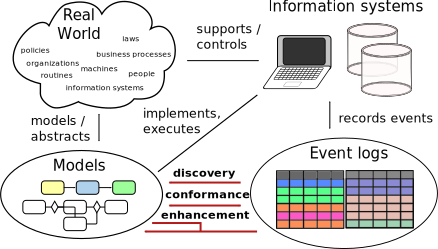
\includegraphics[width=0.55\linewidth]{figures/process-mining-big-picture}
	\caption{The process mining framework Adapted from \citep{VanderAalst2016b}.}
	\label{fig:process-mining}
\end{figure}



%Nevertheless, process mining algorithms work with structured data~\citep{van2005prom, Verbeek2011}. 

\subsection{Contribution to the research questions} 

Several works in the area of \gls{pm} have tackled the problem by transforming it into a \gls{pm} problem. 
%These works enrich \gls{vcs} log data with case and activity information, and then use process mining to discover a model. In this category, Kindler et al.~\citep{kindler2006activity,kindler2006incremental} can discover a Petri net from a structured and enriched version control log. This approach was further improved by Rubin et al.~\citep{rubin2007process} and a ProM\footnote{\url{http://www.promtools.org}} plug-in was provided. Poncin et al.~\citep{Poncin2011a} provide the FRASR framework for preprocessing software repositories such that they can be used in ProM. Song et al.~\citep{Song2007} help addressing the time perspective by mining a dotted chart.
Consequently, approaches have been developed to preprocess VCS data such that \gls{pm} techniques can be applied, and hence, a business process can be derived from the log data.
In this group, \citep{kindler2006activity,kindler2006incremental} developed an algorithm for extracting software processes that are mapped to Petri Nets. Activities, which are not explicit in the logs, are discovered from their input and output artifacts. However, strong assumptions are made on the filenames as well as on the software process lifecycle. %(always design, code, review, testres). Activities (which are not explicit in the logs, like in our case) are discovered from their input and output artifacts. Here defined as triples $<I,O,R>$ where I=input, O=Output, R=resouce who perfomed it.
\citep{rubin2007process} addressed the problem of engineering processes that are not well documented and are usually unstructured. They provided a bridge from Kindler et al.'s approach to ProM \citep{van2005prom} in order to mine different process perspectives, such as performance social network analyses. %but not from a project point of view.
\citep{rubin2014agile} applied \gls{pm} to the touristic industry and obtained user processes from web client logs pursuing the goal of improving the software system by analyzing the underlying process.
\citep{Poncin2011a} developed the FRASR framework for preprocessing software repositories to transform the VCS data to logs that conform to the \gls{pm} event log meta model~\citep{van2005meta} as utilized in ProM \citep{van2005prom}.
However, these approaches disregard the single-instance nature of project-oriented business processes and treat them as procedures that can be repeated over time.
Process mining techniques are related to all the research questions of this thesis. Especially, process discovery helps with addressing \textbf{RQ4}.

\subsection{Limitations} 
While providing interesting insights, these contributions leave out many important aspects of software development projects, such as trying to understand whether the process was done according to the organization plan. Especially, they are limited to either simply display one perspective of the process~\citep{Song2007} or transform the events from software repositories into the standard \gls{xes} format which can be mined by tools like ProM. In this case, existing methods only take into account high level information (such as the type of file) to label events accordingly. Textual information is also taken into account \citep{rubin2007process} but often limited to use of a dictionary for identifying keywords. Moreover, fine granular information on the amount of change and the comments of commit messages have not been exploited enough by existing literature.

\todo[inline]{CHECK here! Below goes a summary that tells what process mining techniques are relevant}

Process mining methods work with event logs. 

All types process mining are useful when it comes to analysing historical data. 

There are works that show their applicability to software development. However, software development data is not an input and that can be directly consumed by process mining algorithms. Hence, manual work or techniques to transform development data into an event log are needed. 

\section{Mining Software Repositories}
\label{sec:msr}






Relevant approaches in the area of mining software repositories (a software engineering branch), are the following.

Automatic capturing of events from software development. 
Gousios et al. provide a technique to extract events from GitHub and store them into a database. This involves defining a schema to capture the various entities that constitute an atomic change event in the software.

These area is used as the base for providing techniques and algorithms as solutions to engineering problems. These problems revolve around questions aimed at understanding various performance and functionality issues with the software at several stages. 

\section{Software Visualization}
\label{sec:visualization}

Software visualisation techniques include

- HPI visual software analytics 
- Software as cities
- Graph visualisations (e.g., social network analyses, static and dynamic graphs, )
- Plots and charts (Dashboards)
- Kanban/Project management KPI visualisations

\section{Text Mining}
\label{sec:text-mining}

%\subsection{Description of the field} 

\Gls{tm} refers to the process of deriving information from natural language text. It relates to data mining in the aspect that both strive to extract meaningful information from raw data. However, data mining is characterized as the extraction of implicit, previously unknown, and potentially useful information from data, whereas with text mining the information to be extracted is clearly and explicitly stated in the text~\citep{Witten2004}. 
\Gls{tm} can be regarded as going beyond information access to further help users analyze and digest information and facilitate decision making. There are also many applications of text mining where the primary goal is to analyze and discover any interesting patterns, including trends and outliers in text data.
Although text mining is mostly about \gls{nlp}~\citep{jurafsky2014speech}, it embraces also applications that go beyond. For example, it analyzes linkage structures such as the citations in the academic literature and hyperlinks in the Web literature, both useful sources of information that lie outside the traditional domain of \gls{nlp}. 

%The main types of text mining are the following.
%
%%\Cref{tab:text-mining-overview} gives a compact overview on the types of text mining and some example references.
%%
%%\begin{table}[!h]
\centering
\caption{Overview on text mining types}
\label{tab:text-mining-overview}
\vspace{5pt}
%\resizebox{\textwidth}{!}{
\begin{tabular}{m{4cm}m{5cm}m{4cm}}
\toprule
\textbf{Type}                         & \textbf{Task}                                                                                                                   & \textbf{References}                                                                                           \\ \midrule
Information extraction       & Filling in templates from natural language text                                                                        & \cite{cowie1996information}, \cite{mooney1999relational}, \cite{seymore1999learning}, \cite{banko2007open} \\ %\midrule
Topic detection and tracking & Finding and following new events in a stream                                                                           & \cite{Allan1998}, \cite{wayne2000multilingual}                                                  \\ %\midrule
Summarization                & Reducing the content obtained from text documents, still keeping the topic                                             & \cite{aggarwal2012mining}, \cite{gupta2009survey}                                                    \\ %\midrule
Categorization               & Identifying the main themes of a document                                                                              & \cite{sebastiani2002machine}, \cite{joachims1998text}                                                \\ %\midrule
Clustering                   & Group similar documents by predefined topics                                                                           & \cite{zhao2001criterion}, \cite{fung2003hierarchical}, \cite{aggarwal2012mining}                     \\ %\midrule
Concept Linkage              & Connect related documents by identifying their shared concepts                                                         & \cite{maedche2000mining}, \cite{fan2006tapping}, \cite{gupta2009survey}                             \\ %\midrule
Information visualization    & Visualizing large textual sources                                                                                      & \cite{wong1999visualizing}, \cite{Mostafa2013}                                                       \\ %\midrule
Question answering           & Automatically answer questions posed by humans                                                                         & \cite{katz1997sentence}, \cite{kwok2001scaling}, \cite{aggarwal2012mining}                           \\ %\midrule
Association rule mining      & Study the relationships and implications among topics or descriptive concepts that are used to characterize a corpus & \cite{agrawal1993mining}, \cite{agrawal1994fast}, \cite{hu2010}                                      \\ \bottomrule
\end{tabular}
%}
\end{table}
%
%\begin{description}
%	\item[Information extraction.] 
%%	Information extraction is used to refer to the task of filling in templates from natural language text. The goal is to extract from the documents (which may be in a variety of languages) salient facts about prespecified types of events, entities or relationships. These facts are then usually entered automatically into a database, which may then be used to analyze the data for trends, to give a natural language summary, or simply to serve for on-line access. Traditional information extraction techniques~\citep{cowie1996information,mooney1999relational} leverage on rule-based systems that match predefined linguistic patterns. More recently, work on named entity recognition uses statistical machine learning methods~\citep{seymore1999learning}. A tool that uses unsupervised learning can be found in \citep{banko2007open}.
%	It is the task of filling in templates from natural language text. The goal is to extract from the documents (which may be in a variety of languages) salient facts about prespecified types of events, entities or relationships. They can be used to analyze the data for trends, to give a natural language summary, or simply to serve for on-line access. Typical examples can be found in~\citep{cowie1996information,mooney1999relational,seymore1999learning,banko2007open}.
%	
%	\item[Topic detection and tracking.] 
%%	\Gls{tdt} was a DARPA-sponsored initiative to investigate on finding and following new events in a stream of broadcast news stories. The \gls{tdt} problem consists of three major tasks: (1) \emph{segmenting} a stream of data, especially recognized speech, into distinct stories; (2) \emph{identifying} those news stories that are the first to discuss a new event occurring in the news; and (3) given a small number of sample news stories about an event, \emph{finding} all \emph{following} stories in the stream.
%%	The work of \citep{allan2002introduction} has formally defined this problem and proposed the initial set of algorithms for the task. Main subtasks of TDT, as identified in \citep{wayne2000multilingual} are 
%%	(i) finding topically homogeneous regions (segmentation); (ii) finding additional stories about a given topic (tracking); (iii) detecting and threading together new topics (detection); (iv) Detecting new topics (first story detection); and (v) Deciding whether stories are on the same topic (linking). An example of a real-world TDT system is Google Alerts\footnote{\url{https://www.google.com/alerts}}.
%	The \gls{tdt} problem consists of three major tasks: (1) \emph{segmenting} a stream of data, especially recognized speech, into distinct stories; (2) \emph{identifying} those news stories that are the first to discuss a new event occurring in the news; and (3) given a small number of sample news stories about an event, \emph{finding} all \emph{following} stories in the stream.
%	Typical examples can be found in~\citep{wayne2000multilingual,allan2002introduction}.
%	%	The work of \citep{allan2002introduction} has formally defined this problem and proposed the initial set of algorithms for the task. Main subtasks of TDT, as identified in \citep{wayne2000multilingual} are 
%	%	(i) finding topically homogeneous regions (segmentation); (ii) finding additional stories about a given topic (tracking); (iii) detecting and threading together new topics (detection); (iv) Detecting new topics (first story detection); and (v) Deciding whether stories are on the same topic (linking). An example of a real-world TDT system is Google Alerts\footnote{\url{https://www.google.com/alerts}}.
%	
%	\item[Summarization.] 
%%	Summarization is the task of reducing the content obtained from text documents, still keeping a brief overview on a topic that they treat. Summarization techniques generally fall into two categories \citep{Aggarwal2015}. In extractive summarization, a summary consists of information units extracted from the original text; in contrast, in abstractive summarization, a summary may contain {\textquotedblleft synthesized\textquotedblright} information units that may not necessarily occur in the text document. An automatic summarization process can be divided into three steps \citep{gupta2009survey}: (1) the \emph{preprocessing} step where a structured representation of the original text is obtained; (2) the \emph{processing} step where an algorithm must transform the text structure into a summary structure; and (3) the \emph{generation} step where the final summary is obtained from the summary structure. 
%%	A plethora of text summarization tools can be found online. A few examples are the open source libraries such Open Text Summarizer\footnote{\url{https://www.splitbrain.org/services/ots}}, Sumplify\footnote{\url{http://sumplify.com/}} and Online summarize tool\footnote{\url{http://www.tools4noobs.com/summarize/}}.
%Summarization is the task of reducing the content obtained from text documents, still keeping a brief overview on a topic that they treat. Typical examples of can be found in~\citep{gupta2009survey,Aggarwal2015}. Some open source libraries are Open Text Summarizer\footnote{\url{https://www.splitbrain.org/services/ots}}, Sumplify\footnote{\url{http://sumplify.com/}} and Online summarize tool\footnote{\url{http://www.tools4noobs.com/summarize/}}.
%	
%	\item[Categorization.] 
%%	Categorization aims at identifying the main themes of a document. This translates into assigning natural language documents to predefined categories according to their content~\citep{sebastiani2002machine}. Categorization often relies on a thesaurus for which topics are predefined, and relationships are identified by looking for broad terms, narrower terms, synonyms, and related terms. \Glspl{svm} are used to automatically learn text classifiers from examples~\citep{joachims1998text}. Categorization tools usually rank documents according to how much of their content fits in a particular topic. 
%%	
%	Categorization aims at assigning natural language documents to predefined categories according to their content. 
%%	Categorization often relies on a thesaurus for which topics are predefined, and relationships are identified by looking for broad terms, narrower terms, synonyms, and related terms. 
%	\Glspl{svm} are used to automatically learn text classifiers from examples. Typical examples can be found in~\citep{joachims1998text,sebastiani2002machine}.
%%	Categorization tools usually rank documents according to how much of their content fits in a particular topic. 
%	
%	\item[Clustering.] 
%%	Clustering is a technique used to group similar documents, but it differs from categorization in that documents are clustered on the fly instead of through predefined topics. Documents can also appear in multiple subtopics, ensuring that useful documents are not omitted from the search results. A basic clustering algorithm creates a vector of topics for each document and measures the weights of how the document fits into each cluster. A survey of clustering algorithms can be found in \citep{Aggarwal2015}. 
%	Clustering is a technique used to group similar documents, but it differs from categorization in that documents are clustered on the fly instead of through predefined topics. 
%%	Documents can also appear in multiple subtopics, ensuring that useful documents are not omitted from the search results. A basic clustering algorithm creates a vector of topics for each document and measures the weights of how the document fits into each cluster. 
%A literature review of clustering algorithms can be found in \citep{Aggarwal2015}. 
%	
%	\item[Concept Linkage.] 
%%	Concept-linkage tools connect related documents by identifying their shared concepts, helping users find information they perhaps would not have found through traditional search methods~\citep{gupta2009survey}. It promotes browsing for information rather than searching for it. For example, a text mining software solution may easily identify a transitive closure in a set of topics \{X, Y, Z\}, i.e., a link between X and Y, a link between Y and Z, %. But the text mining tool could also detect a potential 	and a link between X and Z. %(i.e. transitive closure on the set of topics), something that a human researcher has not come across yet.	With large sets of data, such a relationship could be disregarded by humans. %because of the large volume of information s/he would have to sort through to make the connection.
%	Concept-linkage tools connect related documents by identifying their shared concepts, helping users find information they perhaps would not have found through traditional search methods. Typical examples can be found in~\citep{gupta2009survey}. 
%%	It promotes browsing for information rather than searching for it. For example, a text mining software solution may easily identify a transitive closure in a set of topics \{X, Y, Z\}, i.e., a link between X and Y, a link between Y and Z, %. But the text mining tool could also detect a potential 
%%	and a link between X and Z. %(i.e. transitive closure on the set of topics), something that a human researcher has not come across yet 
%%	With large sets of data, such a relationship could be disregarded by humans. %because of the large volume of information s/he would have to sort through to make the connection.
%	
%	\item[Information Visualization.] 
%%	Information visualization aims at visualizing large textual sources in such a way that the content can be displayed in a hierarchy or map and provides browsing features, in addition to simple search. For instance, governments or police can identify terrorist networks in a map and identify crimes that were previously unconnected~\citep{gupta2009survey}.
%	Information visualization aims at visualizing large textual sources in such a way that the content can be displayed in a hierarchy or map and provides browsing features, in addition to simple search. Typical examples can be found in~\citep{gupta2009survey}.
%	
%	\item[Question Answering.] 
%%	Another application area of developed text-mining technologies, along with the natural language processing, is natural language features Question Answering (QA). QA is concerned with building systems that automatically answer questions posed by humans in a natural language.
%%	One of the first Query Answering tools was START\footnote{\url{http://start.csail.mit.edu/index.php}}, developed in the work of \citep{katz1997sentence}. Question answering has been extensively used in Biomedical domain for aiding researchers and health care professionals in managing the continuous growth of information.	
%%	Another application area of developed text-mining technologies, along with the natural language processing, is natural language features Question Answering (QA). 
%	QA is concerned with building systems that automatically answer questions posed by humans in a natural language. One of the first Query Answering tools was START\footnote{\url{http://start.csail.mit.edu/index.php}}, developed in the work of \citep{katz1997sentence}. 
%%	Question answering has been extensively used in Biomedical domain for aiding researchers and health care professionals in managing the continuous growth of information.
%	
%	\item[Association Rule Mining.] 
%%	The focus of association rules mining is to study the relationships and implications among topics, or descriptive concepts, that are used to characterize a corpus. The work of \citep{agrawal1994fast} shows how it is possible to discover association rules from massive data from databases, referred to as \emph{basket} data. The same approach can be followed by constructing a database of rules using information extraction methods and subsequently applying techniques, e.g. \citep{hu2010}, to uncover hidden associations in the database. For instance, a rule might be that 98\% of customers that purchase tires and auto accessories also get automotive services done. This suggests that association rules can be captured as if/then patterns. Criteria such as support and confidence~\citep{agrawal1993mining} are used to identify the most important relationships. Support is an indication of how frequently the items appear in the database. Confidence indicates the number of times the if/then statements has been found to be true.
%	The focus of association rules mining is to study the relationships and implications among topics, or descriptive concepts, that are used to characterize a corpus. Typical examples can be found in~\citep{agrawal1993mining,agrawal1994fast,hu2010}.
%%	The work of \citep{agrawal1994fast} shows how it is possible to discover association rules from massive data from databases, referred to as \emph{basket} data. The same approach can be followed by constructing a database of rules using information extraction methods and subsequently applying techniques, e.g. \citep{hu2010}, to uncover hidden associations in the database. For instance, a rule might be that 98\% of customers that purchase tires and auto accessories also get automotive services done. This suggests that association rules can be captured as if/then patterns. Criteria such as support and confidence~\citep{agrawal1993mining} are used to identify the most important relationships. Support is an indication of how frequently the items appear in the database. Confidence indicates the number of times the if/then statements has been found to be true.
%	
%\end{description}

\subsection{Contribution to the research questions} 

%\todoinline{more details}

%My research involves unstructured data in the form of word processor documents, emails, user forums, and commit messages from \gls{vcs}. Text mining algorithms can be combined to quantitative data to gather information about project work. For example, topics models can be combined to time-clustered messages from pull request comments. In this way it is possible order to discover ``hot topics" (e.g. deliverable, milestone, meeting, etc) during project development. More in general, text mining techniques help with preprocessing the data and retrieving relevant information. Successively, this information can be brought together to create a structured event log in the \gls{xes} format. Therefore, text mining research serves and a preprocessing technique to facilitate process extraction. Especially, it helps as follows. 

\gls{nlp} based approaches have been used to identify process cases and activities. Contributions in this group the have focused on process discovery. \citep{Goncalves2009a} discovered a model from group stories. \citep{Friedrich2011} reaches 77\% of accuracy in reconstructing process models from text. \citep{DoNascimento2012} analyze legacy systems code to infer business process rules and activities. \citep{DiCiccio2013} use \gls{nlp} to aid the extraction of artful processes from knowledge workers emails.

There are also works that help with information extraction. \citep{Maalej2010} use \gls{nlp} for automating descriptions of work sessions by analyzing developers' informal text notes about their tasks. Developers are then classified into two classes based on their behavior: developers who use problem information to refer to their current activity and developers who refer to task and requirements. \citep{Kouters2012} developed an identity merging algorithm based on Latent Semantic Analysis (LSA) to disambiguate user emails. \citep{Licorish2014} mined developer comments to understand their attitudes.

Role discovery has also seen contributions. A number of algorithms have been developed to mine roles from \gls{rbac} systems alone (\citep{Lu2015,frank2013role}) or combining their data with process history logs, as in ~\citep{baumgrass2012deriving}. A survey of existing techniques and algorithms can be found in \citep{Mitra2016}.

This body of works 
%suggests that process insights can be obtained from unstructured data. \Gls{tm} supports my research with preprocessing to facilitate process extraction. Especially, it 
helps with:
\begin{inparaenum}[\itshape i)]
	\item \textbf{RQ2} -- extracting case characteristics from conversations in user forums;
	\item \textbf{RQ3} -- extracting resource roles from user comments in commit messages;
	\item \textbf{RQ4} -- extracting activities out of coordination message exchanges.
\end{inparaenum} 

\subsection{Limitations}
\Gls{tm} techniques do not natively support extraction of processes, but they can be used to help addressing information extraction from unstructured data. \Gls{tm} approaches focus on obtaining structured information from unstructured textual data, and mainly uses \gls{nlp}~\citep{Witten:1999}. Works that use \gls{nlp} can be found in both \gls{pm} \citep{VanderAalst2016b} and \gls{msr} \citep{Chen2016a}. In the \gls{bpm} \citep{Dumas2018} area, \gls{nlp} techniques have been used to understand process activities~\citep{Leopold2013,Mendling2014} and analyze software processes under a knowledge-intensive perspective~\citep{DeA.R.Goncalves2011,Richetti2017}. Likewise, in the~\gls{msr} area, \gls{nlp} has been used as an information extraction tool to obtain informative metrics from a software engineering perspective~\citep{Thomas2014,Chen2016a}. 

\todo[inline]{CHECK! As with the previous section}

Text mining techniques include state of the art NLP methods to extract knowledge from unstructured data. These methods exploit the communication channels used by developers. Such unstructured data is rich in information. 
Relevant techniques focus on these data.
Any technique is enriching the event log using these data?

\section{Summary of Relevant Techniques}
\label{sec:summary-of-relevant-techniques}

\todo[inline]{Here go the techniques relevant for this thesis.} 

This research combines ideas from the above mentioned areas to devise algorithms for mining the software development process. This section defines the contribution of related fields to the four research question. \Cref{table:literature-classification} lists summarizes the most relevant works in the literature and classifies them in relation the addressed research questions.

% Please add the following required packages to your document preamble:
% \usepackage{booktabs}
\begin{table}[]
%\vspace*{-\baselineskip}
\centering
\caption{Classification of existing literature addressing the various aspects of mining the development process}
\label{table:literature-classification}
\begin{tabular}{@{}c>{\raggedright}m{3cm}>{\raggedright}m{2.5cm}>{\raggedright}m{2.5cm}>{\raggedright\arraybackslash}m{2.5cm}@{}}
\toprule
\multicolumn{1}{l}{} & \textbf{R1}                                              & \textbf{R2}                                                                                               & \textbf{R3} & \textbf{R4}                                      \\ \midrule

\textbf{PM} & Dotted Chart \citep{Song2007} & Decision mining \citep{Rozinat2006} & Visualization techniques \citep{Baumgrass2013} Organizational mining \citep{Song2008} \citep{Schonig2015} & Bug fixing \citep{Poncin2011a}, Workflow fragments \citep{DBLP:conf/se/KindlerRS06,kindler2006incremental} \\ \midrule
\textbf{TM} & Information extraction \citep{cowie1996information} & Topic models \citep{Chen2016a} Theory-generating case studies \citep{Lindberg2016} & Social network \citep{Bird2006} Survey \citep{Begel2010} \citep{DeA.R.Goncalves2010} & Speech acts \citep{DiCiccio2013a} \citep{Campos2018} Natural language processing \citep{Friedrich2011} \\ \midrule
\textbf{MSR} & Time series \citep{Ruohonen2015} \citep{Hou2014}, Statistical analyses \citep{Oliva2011} & Network analysis \citep{DAmbros2009}, \citep{Zimmermann2008}, Language Models \citep{Allamanis2013} & Email analysis \citep{Bird2006}, Role identification \citep{Yu.LiguoRamaswamy.2007} & Exploratory studies \citep{Gousios2014} \\ \bottomrule
\end{tabular}
\vspace*{-\baselineskip}
\end{table}

